% Created by tikzDevice version 0.9 on 2016-01-12 22:38:47
% !TEX encoding = UTF-8 Unicode
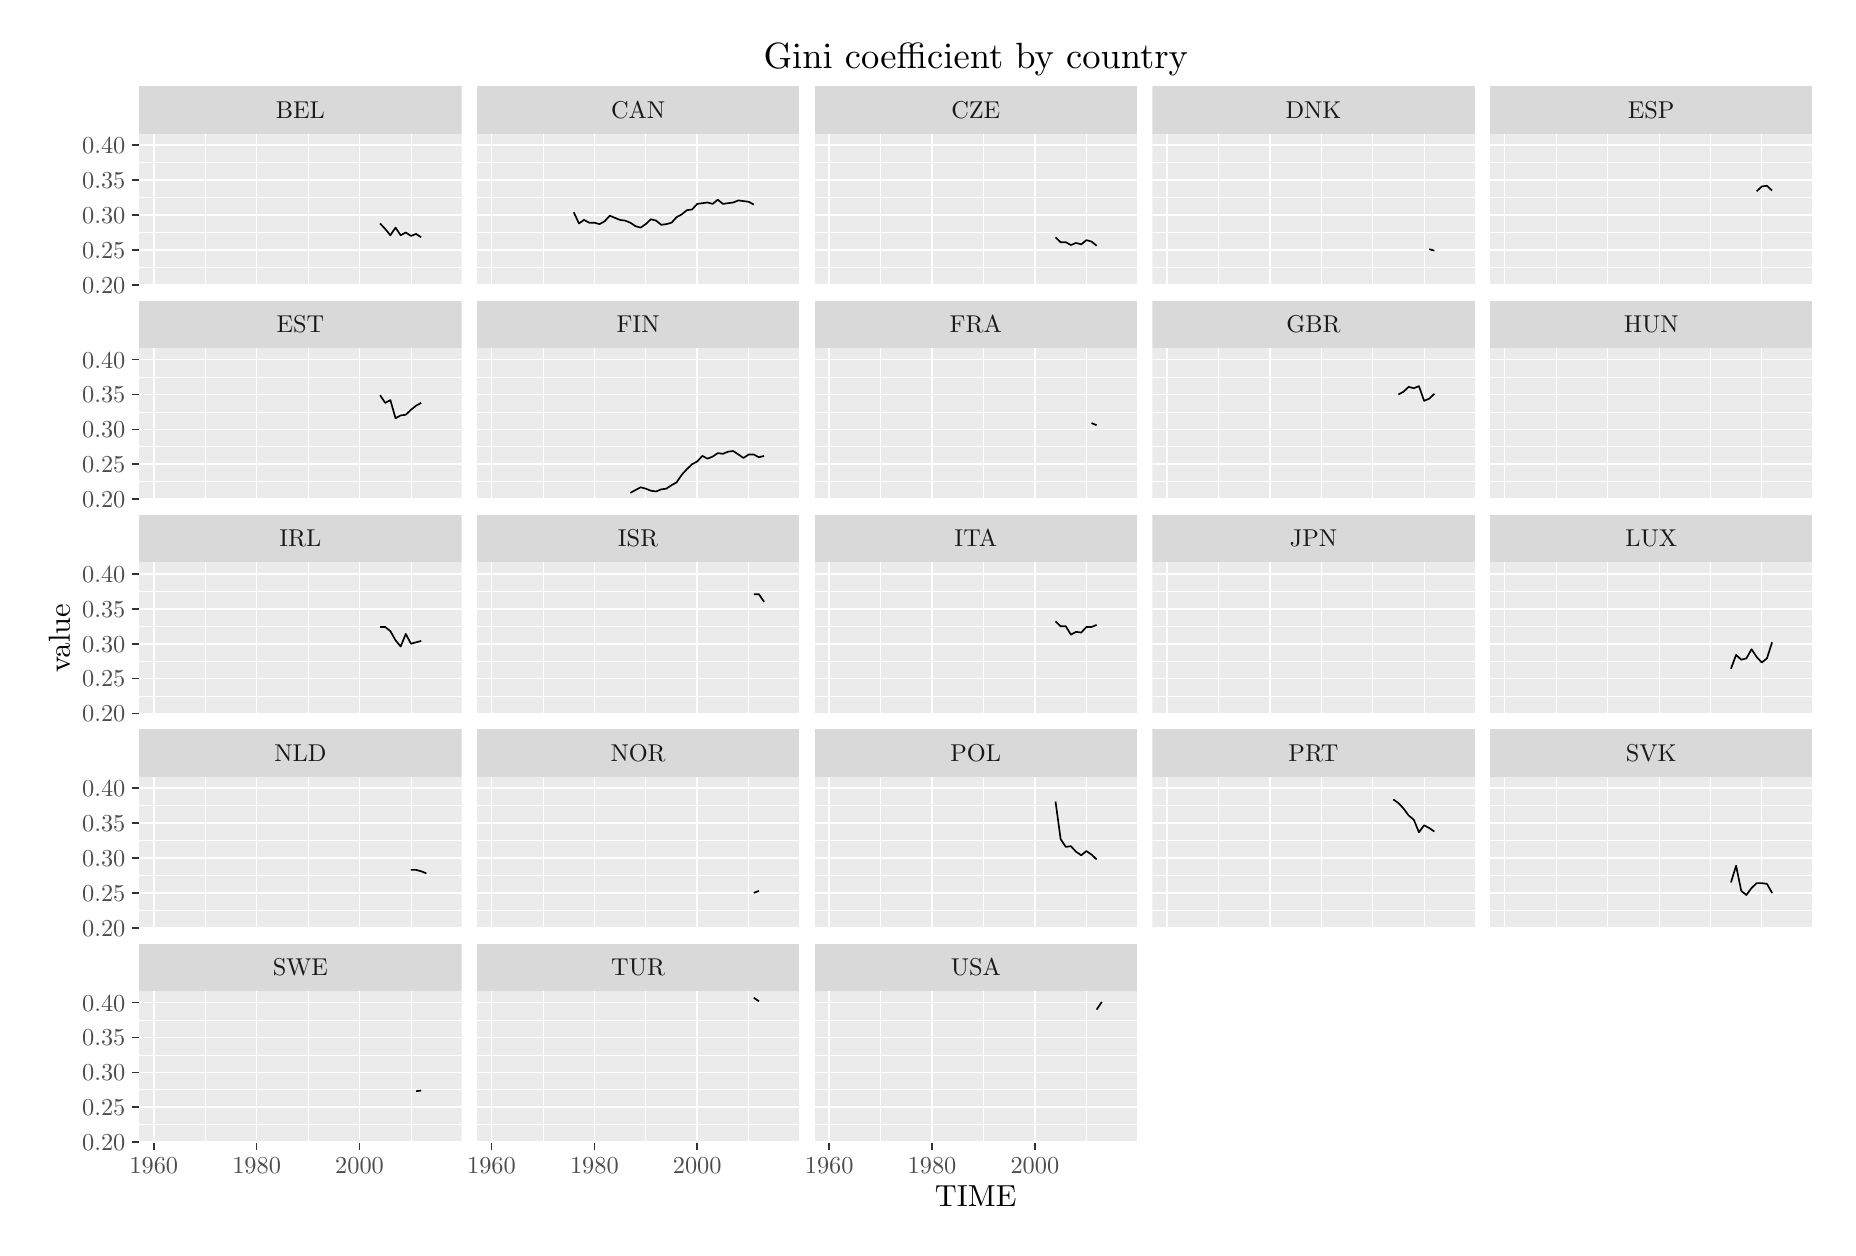
\begin{tikzpicture}[x=1pt,y=1pt]
\definecolor{fillColor}{RGB}{255,255,255}
\path[use as bounding box,fill=fillColor,fill opacity=0.00] (0,0) rectangle (650.43,433.62);
\begin{scope}
\path[clip] (  0.00,  0.00) rectangle (650.43,433.62);
\definecolor{drawColor}{RGB}{255,255,255}
\definecolor{fillColor}{RGB}{255,255,255}

\path[draw=drawColor,line width= 0.6pt,line join=round,line cap=round,fill=fillColor] (  0.00,  0.00) rectangle (650.43,433.62);
\end{scope}
\begin{scope}
\path[clip] ( 40.27,340.48) rectangle (156.80,395.37);
\definecolor{fillColor}{gray}{0.92}

\path[fill=fillColor] ( 40.27,340.48) rectangle (156.80,395.37);
\definecolor{drawColor}{RGB}{255,255,255}

\path[draw=drawColor,line width= 0.3pt,line join=round] ( 40.27,347.01) --
	(156.80,347.01);

\path[draw=drawColor,line width= 0.3pt,line join=round] ( 40.27,359.61) --
	(156.80,359.61);

\path[draw=drawColor,line width= 0.3pt,line join=round] ( 40.27,372.21) --
	(156.80,372.21);

\path[draw=drawColor,line width= 0.3pt,line join=round] ( 40.27,384.81) --
	(156.80,384.81);

\path[draw=drawColor,line width= 0.3pt,line join=round] ( 64.15,340.48) --
	( 64.15,395.37);

\path[draw=drawColor,line width= 0.3pt,line join=round] (101.32,340.48) --
	(101.32,395.37);

\path[draw=drawColor,line width= 0.3pt,line join=round] (138.49,340.48) --
	(138.49,395.37);

\path[draw=drawColor,line width= 0.6pt,line join=round] ( 40.27,340.71) --
	(156.80,340.71);

\path[draw=drawColor,line width= 0.6pt,line join=round] ( 40.27,353.31) --
	(156.80,353.31);

\path[draw=drawColor,line width= 0.6pt,line join=round] ( 40.27,365.91) --
	(156.80,365.91);

\path[draw=drawColor,line width= 0.6pt,line join=round] ( 40.27,378.51) --
	(156.80,378.51);

\path[draw=drawColor,line width= 0.6pt,line join=round] ( 40.27,391.11) --
	(156.80,391.11);

\path[draw=drawColor,line width= 0.6pt,line join=round] ( 45.56,340.48) --
	( 45.56,395.37);

\path[draw=drawColor,line width= 0.6pt,line join=round] ( 82.74,340.48) --
	( 82.74,395.37);

\path[draw=drawColor,line width= 0.6pt,line join=round] (119.91,340.48) --
	(119.91,395.37);
\definecolor{drawColor}{RGB}{0,0,0}

\path[draw=drawColor,line width= 0.6pt,line join=round] (127.34,362.88) --
	(129.20,360.87) --
	(131.06,358.60) --
	(132.92,361.37) --
	(134.78,358.60) --
	(136.63,359.61) --
	(138.49,358.35) --
	(140.35,359.10) --
	(142.21,357.84);
\end{scope}
\begin{scope}
\path[clip] (162.30,340.48) rectangle (278.83,395.37);
\definecolor{fillColor}{gray}{0.92}

\path[fill=fillColor] (162.30,340.48) rectangle (278.83,395.37);
\definecolor{drawColor}{RGB}{255,255,255}

\path[draw=drawColor,line width= 0.3pt,line join=round] (162.30,347.01) --
	(278.83,347.01);

\path[draw=drawColor,line width= 0.3pt,line join=round] (162.30,359.61) --
	(278.83,359.61);

\path[draw=drawColor,line width= 0.3pt,line join=round] (162.30,372.21) --
	(278.83,372.21);

\path[draw=drawColor,line width= 0.3pt,line join=round] (162.30,384.81) --
	(278.83,384.81);

\path[draw=drawColor,line width= 0.3pt,line join=round] (186.18,340.48) --
	(186.18,395.37);

\path[draw=drawColor,line width= 0.3pt,line join=round] (223.35,340.48) --
	(223.35,395.37);

\path[draw=drawColor,line width= 0.3pt,line join=round] (260.53,340.48) --
	(260.53,395.37);

\path[draw=drawColor,line width= 0.6pt,line join=round] (162.30,340.71) --
	(278.83,340.71);

\path[draw=drawColor,line width= 0.6pt,line join=round] (162.30,353.31) --
	(278.83,353.31);

\path[draw=drawColor,line width= 0.6pt,line join=round] (162.30,365.91) --
	(278.83,365.91);

\path[draw=drawColor,line width= 0.6pt,line join=round] (162.30,378.51) --
	(278.83,378.51);

\path[draw=drawColor,line width= 0.6pt,line join=round] (162.30,391.11) --
	(278.83,391.11);

\path[draw=drawColor,line width= 0.6pt,line join=round] (167.60,340.48) --
	(167.60,395.37);

\path[draw=drawColor,line width= 0.6pt,line join=round] (204.77,340.48) --
	(204.77,395.37);

\path[draw=drawColor,line width= 0.6pt,line join=round] (241.94,340.48) --
	(241.94,395.37);
\definecolor{drawColor}{RGB}{0,0,0}

\path[draw=drawColor,line width= 0.6pt,line join=round] (197.33,366.92) --
	(199.19,362.88) --
	(201.05,364.14) --
	(202.91,363.14) --
	(204.77,363.14) --
	(206.63,362.63) --
	(208.48,363.64) --
	(210.34,365.66) --
	(212.20,364.90) --
	(214.06,364.14) --
	(215.92,363.89) --
	(217.78,363.14) --
	(219.64,361.88) --
	(221.49,361.37) --
	(223.35,362.63) --
	(225.21,364.40) --
	(227.07,363.89) --
	(228.93,362.38) --
	(230.79,362.63) --
	(232.65,363.14) --
	(234.50,365.15) --
	(236.36,366.16) --
	(238.22,367.67) --
	(240.08,367.92) --
	(241.94,369.94) --
	(243.80,370.19) --
	(245.66,370.44) --
	(247.52,369.94) --
	(249.37,371.45) --
	(251.23,369.94) --
	(253.09,370.19) --
	(254.95,370.44) --
	(256.81,371.20) --
	(258.67,370.95) --
	(260.53,370.70) --
	(262.38,369.69);
\end{scope}
\begin{scope}
\path[clip] (284.33,340.48) rectangle (400.86,395.37);
\definecolor{fillColor}{gray}{0.92}

\path[fill=fillColor] (284.33,340.48) rectangle (400.86,395.37);
\definecolor{drawColor}{RGB}{255,255,255}

\path[draw=drawColor,line width= 0.3pt,line join=round] (284.33,347.01) --
	(400.86,347.01);

\path[draw=drawColor,line width= 0.3pt,line join=round] (284.33,359.61) --
	(400.86,359.61);

\path[draw=drawColor,line width= 0.3pt,line join=round] (284.33,372.21) --
	(400.86,372.21);

\path[draw=drawColor,line width= 0.3pt,line join=round] (284.33,384.81) --
	(400.86,384.81);

\path[draw=drawColor,line width= 0.3pt,line join=round] (308.21,340.48) --
	(308.21,395.37);

\path[draw=drawColor,line width= 0.3pt,line join=round] (345.39,340.48) --
	(345.39,395.37);

\path[draw=drawColor,line width= 0.3pt,line join=round] (382.56,340.48) --
	(382.56,395.37);

\path[draw=drawColor,line width= 0.6pt,line join=round] (284.33,340.71) --
	(400.86,340.71);

\path[draw=drawColor,line width= 0.6pt,line join=round] (284.33,353.31) --
	(400.86,353.31);

\path[draw=drawColor,line width= 0.6pt,line join=round] (284.33,365.91) --
	(400.86,365.91);

\path[draw=drawColor,line width= 0.6pt,line join=round] (284.33,378.51) --
	(400.86,378.51);

\path[draw=drawColor,line width= 0.6pt,line join=round] (284.33,391.11) --
	(400.86,391.11);

\path[draw=drawColor,line width= 0.6pt,line join=round] (289.63,340.48) --
	(289.63,395.37);

\path[draw=drawColor,line width= 0.6pt,line join=round] (326.80,340.48) --
	(326.80,395.37);

\path[draw=drawColor,line width= 0.6pt,line join=round] (363.97,340.48) --
	(363.97,395.37);
\definecolor{drawColor}{RGB}{0,0,0}

\path[draw=drawColor,line width= 0.6pt,line join=round] (371.41,357.84) --
	(373.26,356.08) --
	(375.12,356.08) --
	(376.98,355.07) --
	(378.84,355.83) --
	(380.70,355.32) --
	(382.56,356.84) --
	(384.42,356.33) --
	(386.27,354.82);
\end{scope}
\begin{scope}
\path[clip] (406.36,340.48) rectangle (522.90,395.37);
\definecolor{fillColor}{gray}{0.92}

\path[fill=fillColor] (406.36,340.48) rectangle (522.90,395.37);
\definecolor{drawColor}{RGB}{255,255,255}

\path[draw=drawColor,line width= 0.3pt,line join=round] (406.36,347.01) --
	(522.90,347.01);

\path[draw=drawColor,line width= 0.3pt,line join=round] (406.36,359.61) --
	(522.90,359.61);

\path[draw=drawColor,line width= 0.3pt,line join=round] (406.36,372.21) --
	(522.90,372.21);

\path[draw=drawColor,line width= 0.3pt,line join=round] (406.36,384.81) --
	(522.90,384.81);

\path[draw=drawColor,line width= 0.3pt,line join=round] (430.25,340.48) --
	(430.25,395.37);

\path[draw=drawColor,line width= 0.3pt,line join=round] (467.42,340.48) --
	(467.42,395.37);

\path[draw=drawColor,line width= 0.3pt,line join=round] (504.59,340.48) --
	(504.59,395.37);

\path[draw=drawColor,line width= 0.6pt,line join=round] (406.36,340.71) --
	(522.90,340.71);

\path[draw=drawColor,line width= 0.6pt,line join=round] (406.36,353.31) --
	(522.90,353.31);

\path[draw=drawColor,line width= 0.6pt,line join=round] (406.36,365.91) --
	(522.90,365.91);

\path[draw=drawColor,line width= 0.6pt,line join=round] (406.36,378.51) --
	(522.90,378.51);

\path[draw=drawColor,line width= 0.6pt,line join=round] (406.36,391.11) --
	(522.90,391.11);

\path[draw=drawColor,line width= 0.6pt,line join=round] (411.66,340.48) --
	(411.66,395.37);

\path[draw=drawColor,line width= 0.6pt,line join=round] (448.83,340.48) --
	(448.83,395.37);

\path[draw=drawColor,line width= 0.6pt,line join=round] (486.00,340.48) --
	(486.00,395.37);
\definecolor{drawColor}{RGB}{0,0,0}

\path[draw=drawColor,line width= 0.6pt,line join=round] (506.45,353.56) --
	(508.31,353.06);
\end{scope}
\begin{scope}
\path[clip] (528.40,340.48) rectangle (644.93,395.37);
\definecolor{fillColor}{gray}{0.92}

\path[fill=fillColor] (528.40,340.48) rectangle (644.93,395.37);
\definecolor{drawColor}{RGB}{255,255,255}

\path[draw=drawColor,line width= 0.3pt,line join=round] (528.40,347.01) --
	(644.93,347.01);

\path[draw=drawColor,line width= 0.3pt,line join=round] (528.40,359.61) --
	(644.93,359.61);

\path[draw=drawColor,line width= 0.3pt,line join=round] (528.40,372.21) --
	(644.93,372.21);

\path[draw=drawColor,line width= 0.3pt,line join=round] (528.40,384.81) --
	(644.93,384.81);

\path[draw=drawColor,line width= 0.3pt,line join=round] (552.28,340.48) --
	(552.28,395.37);

\path[draw=drawColor,line width= 0.3pt,line join=round] (589.45,340.48) --
	(589.45,395.37);

\path[draw=drawColor,line width= 0.3pt,line join=round] (626.62,340.48) --
	(626.62,395.37);

\path[draw=drawColor,line width= 0.6pt,line join=round] (528.40,340.71) --
	(644.93,340.71);

\path[draw=drawColor,line width= 0.6pt,line join=round] (528.40,353.31) --
	(644.93,353.31);

\path[draw=drawColor,line width= 0.6pt,line join=round] (528.40,365.91) --
	(644.93,365.91);

\path[draw=drawColor,line width= 0.6pt,line join=round] (528.40,378.51) --
	(644.93,378.51);

\path[draw=drawColor,line width= 0.6pt,line join=round] (528.40,391.11) --
	(644.93,391.11);

\path[draw=drawColor,line width= 0.6pt,line join=round] (533.69,340.48) --
	(533.69,395.37);

\path[draw=drawColor,line width= 0.6pt,line join=round] (570.87,340.48) --
	(570.87,395.37);

\path[draw=drawColor,line width= 0.6pt,line join=round] (608.04,340.48) --
	(608.04,395.37);
\definecolor{drawColor}{RGB}{0,0,0}

\path[draw=drawColor,line width= 0.6pt,line join=round] (624.76,374.48) --
	(626.62,376.24) --
	(628.48,376.49) --
	(630.34,374.73);
\end{scope}
\begin{scope}
\path[clip] ( 40.27,263.03) rectangle (156.80,317.92);
\definecolor{fillColor}{gray}{0.92}

\path[fill=fillColor] ( 40.27,263.03) rectangle (156.80,317.92);
\definecolor{drawColor}{RGB}{255,255,255}

\path[draw=drawColor,line width= 0.3pt,line join=round] ( 40.27,269.56) --
	(156.80,269.56);

\path[draw=drawColor,line width= 0.3pt,line join=round] ( 40.27,282.16) --
	(156.80,282.16);

\path[draw=drawColor,line width= 0.3pt,line join=round] ( 40.27,294.76) --
	(156.80,294.76);

\path[draw=drawColor,line width= 0.3pt,line join=round] ( 40.27,307.36) --
	(156.80,307.36);

\path[draw=drawColor,line width= 0.3pt,line join=round] ( 64.15,263.03) --
	( 64.15,317.92);

\path[draw=drawColor,line width= 0.3pt,line join=round] (101.32,263.03) --
	(101.32,317.92);

\path[draw=drawColor,line width= 0.3pt,line join=round] (138.49,263.03) --
	(138.49,317.92);

\path[draw=drawColor,line width= 0.6pt,line join=round] ( 40.27,263.26) --
	(156.80,263.26);

\path[draw=drawColor,line width= 0.6pt,line join=round] ( 40.27,275.86) --
	(156.80,275.86);

\path[draw=drawColor,line width= 0.6pt,line join=round] ( 40.27,288.46) --
	(156.80,288.46);

\path[draw=drawColor,line width= 0.6pt,line join=round] ( 40.27,301.06) --
	(156.80,301.06);

\path[draw=drawColor,line width= 0.6pt,line join=round] ( 40.27,313.66) --
	(156.80,313.66);

\path[draw=drawColor,line width= 0.6pt,line join=round] ( 45.56,263.03) --
	( 45.56,317.92);

\path[draw=drawColor,line width= 0.6pt,line join=round] ( 82.74,263.03) --
	( 82.74,317.92);

\path[draw=drawColor,line width= 0.6pt,line join=round] (119.91,263.03) --
	(119.91,317.92);
\definecolor{drawColor}{RGB}{0,0,0}

\path[draw=drawColor,line width= 0.6pt,line join=round] (127.34,300.81) --
	(129.20,298.04) --
	(131.06,299.04) --
	(132.92,292.49) --
	(134.78,293.50) --
	(136.63,293.75) --
	(138.49,295.52) --
	(140.35,297.03) --
	(142.21,298.04);
\end{scope}
\begin{scope}
\path[clip] (162.30,263.03) rectangle (278.83,317.92);
\definecolor{fillColor}{gray}{0.92}

\path[fill=fillColor] (162.30,263.03) rectangle (278.83,317.92);
\definecolor{drawColor}{RGB}{255,255,255}

\path[draw=drawColor,line width= 0.3pt,line join=round] (162.30,269.56) --
	(278.83,269.56);

\path[draw=drawColor,line width= 0.3pt,line join=round] (162.30,282.16) --
	(278.83,282.16);

\path[draw=drawColor,line width= 0.3pt,line join=round] (162.30,294.76) --
	(278.83,294.76);

\path[draw=drawColor,line width= 0.3pt,line join=round] (162.30,307.36) --
	(278.83,307.36);

\path[draw=drawColor,line width= 0.3pt,line join=round] (186.18,263.03) --
	(186.18,317.92);

\path[draw=drawColor,line width= 0.3pt,line join=round] (223.35,263.03) --
	(223.35,317.92);

\path[draw=drawColor,line width= 0.3pt,line join=round] (260.53,263.03) --
	(260.53,317.92);

\path[draw=drawColor,line width= 0.6pt,line join=round] (162.30,263.26) --
	(278.83,263.26);

\path[draw=drawColor,line width= 0.6pt,line join=round] (162.30,275.86) --
	(278.83,275.86);

\path[draw=drawColor,line width= 0.6pt,line join=round] (162.30,288.46) --
	(278.83,288.46);

\path[draw=drawColor,line width= 0.6pt,line join=round] (162.30,301.06) --
	(278.83,301.06);

\path[draw=drawColor,line width= 0.6pt,line join=round] (162.30,313.66) --
	(278.83,313.66);

\path[draw=drawColor,line width= 0.6pt,line join=round] (167.60,263.03) --
	(167.60,317.92);

\path[draw=drawColor,line width= 0.6pt,line join=round] (204.77,263.03) --
	(204.77,317.92);

\path[draw=drawColor,line width= 0.6pt,line join=round] (241.94,263.03) --
	(241.94,317.92);
\definecolor{drawColor}{RGB}{0,0,0}

\path[draw=drawColor,line width= 0.6pt,line join=round] (217.78,265.53) --
	(219.64,266.53) --
	(221.49,267.54) --
	(223.35,267.04) --
	(225.21,266.28) --
	(227.07,266.03) --
	(228.93,266.79) --
	(230.79,267.04) --
	(232.65,268.30) --
	(234.50,269.31) --
	(236.36,272.08) --
	(238.22,274.10) --
	(240.08,275.86) --
	(241.94,276.87) --
	(243.80,278.88) --
	(245.66,277.88) --
	(247.52,278.63) --
	(249.37,279.89) --
	(251.23,279.64) --
	(253.09,280.40) --
	(254.95,280.65) --
	(256.81,279.39) --
	(258.67,278.13) --
	(260.53,279.39) --
	(262.38,279.39) --
	(264.24,278.38) --
	(266.10,278.88);
\end{scope}
\begin{scope}
\path[clip] (284.33,263.03) rectangle (400.86,317.92);
\definecolor{fillColor}{gray}{0.92}

\path[fill=fillColor] (284.33,263.03) rectangle (400.86,317.92);
\definecolor{drawColor}{RGB}{255,255,255}

\path[draw=drawColor,line width= 0.3pt,line join=round] (284.33,269.56) --
	(400.86,269.56);

\path[draw=drawColor,line width= 0.3pt,line join=round] (284.33,282.16) --
	(400.86,282.16);

\path[draw=drawColor,line width= 0.3pt,line join=round] (284.33,294.76) --
	(400.86,294.76);

\path[draw=drawColor,line width= 0.3pt,line join=round] (284.33,307.36) --
	(400.86,307.36);

\path[draw=drawColor,line width= 0.3pt,line join=round] (308.21,263.03) --
	(308.21,317.92);

\path[draw=drawColor,line width= 0.3pt,line join=round] (345.39,263.03) --
	(345.39,317.92);

\path[draw=drawColor,line width= 0.3pt,line join=round] (382.56,263.03) --
	(382.56,317.92);

\path[draw=drawColor,line width= 0.6pt,line join=round] (284.33,263.26) --
	(400.86,263.26);

\path[draw=drawColor,line width= 0.6pt,line join=round] (284.33,275.86) --
	(400.86,275.86);

\path[draw=drawColor,line width= 0.6pt,line join=round] (284.33,288.46) --
	(400.86,288.46);

\path[draw=drawColor,line width= 0.6pt,line join=round] (284.33,301.06) --
	(400.86,301.06);

\path[draw=drawColor,line width= 0.6pt,line join=round] (284.33,313.66) --
	(400.86,313.66);

\path[draw=drawColor,line width= 0.6pt,line join=round] (289.63,263.03) --
	(289.63,317.92);

\path[draw=drawColor,line width= 0.6pt,line join=round] (326.80,263.03) --
	(326.80,317.92);

\path[draw=drawColor,line width= 0.6pt,line join=round] (363.97,263.03) --
	(363.97,317.92);
\definecolor{drawColor}{RGB}{0,0,0}

\path[draw=drawColor,line width= 0.6pt,line join=round] (384.42,290.73) --
	(386.27,289.97);
\end{scope}
\begin{scope}
\path[clip] (406.36,263.03) rectangle (522.90,317.92);
\definecolor{fillColor}{gray}{0.92}

\path[fill=fillColor] (406.36,263.03) rectangle (522.90,317.92);
\definecolor{drawColor}{RGB}{255,255,255}

\path[draw=drawColor,line width= 0.3pt,line join=round] (406.36,269.56) --
	(522.90,269.56);

\path[draw=drawColor,line width= 0.3pt,line join=round] (406.36,282.16) --
	(522.90,282.16);

\path[draw=drawColor,line width= 0.3pt,line join=round] (406.36,294.76) --
	(522.90,294.76);

\path[draw=drawColor,line width= 0.3pt,line join=round] (406.36,307.36) --
	(522.90,307.36);

\path[draw=drawColor,line width= 0.3pt,line join=round] (430.25,263.03) --
	(430.25,317.92);

\path[draw=drawColor,line width= 0.3pt,line join=round] (467.42,263.03) --
	(467.42,317.92);

\path[draw=drawColor,line width= 0.3pt,line join=round] (504.59,263.03) --
	(504.59,317.92);

\path[draw=drawColor,line width= 0.6pt,line join=round] (406.36,263.26) --
	(522.90,263.26);

\path[draw=drawColor,line width= 0.6pt,line join=round] (406.36,275.86) --
	(522.90,275.86);

\path[draw=drawColor,line width= 0.6pt,line join=round] (406.36,288.46) --
	(522.90,288.46);

\path[draw=drawColor,line width= 0.6pt,line join=round] (406.36,301.06) --
	(522.90,301.06);

\path[draw=drawColor,line width= 0.6pt,line join=round] (406.36,313.66) --
	(522.90,313.66);

\path[draw=drawColor,line width= 0.6pt,line join=round] (411.66,263.03) --
	(411.66,317.92);

\path[draw=drawColor,line width= 0.6pt,line join=round] (448.83,263.03) --
	(448.83,317.92);

\path[draw=drawColor,line width= 0.6pt,line join=round] (486.00,263.03) --
	(486.00,317.92);
\definecolor{drawColor}{RGB}{0,0,0}

\path[draw=drawColor,line width= 0.6pt,line join=round] (495.30,301.06) --
	(497.16,302.07) --
	(499.01,303.83) --
	(500.87,303.33) --
	(502.73,304.08) --
	(504.59,298.79) --
	(506.45,299.55) --
	(508.31,301.31);
\end{scope}
\begin{scope}
\path[clip] (528.40,263.03) rectangle (644.93,317.92);
\definecolor{fillColor}{gray}{0.92}

\path[fill=fillColor] (528.40,263.03) rectangle (644.93,317.92);
\definecolor{drawColor}{RGB}{255,255,255}

\path[draw=drawColor,line width= 0.3pt,line join=round] (528.40,269.56) --
	(644.93,269.56);

\path[draw=drawColor,line width= 0.3pt,line join=round] (528.40,282.16) --
	(644.93,282.16);

\path[draw=drawColor,line width= 0.3pt,line join=round] (528.40,294.76) --
	(644.93,294.76);

\path[draw=drawColor,line width= 0.3pt,line join=round] (528.40,307.36) --
	(644.93,307.36);

\path[draw=drawColor,line width= 0.3pt,line join=round] (552.28,263.03) --
	(552.28,317.92);

\path[draw=drawColor,line width= 0.3pt,line join=round] (589.45,263.03) --
	(589.45,317.92);

\path[draw=drawColor,line width= 0.3pt,line join=round] (626.62,263.03) --
	(626.62,317.92);

\path[draw=drawColor,line width= 0.6pt,line join=round] (528.40,263.26) --
	(644.93,263.26);

\path[draw=drawColor,line width= 0.6pt,line join=round] (528.40,275.86) --
	(644.93,275.86);

\path[draw=drawColor,line width= 0.6pt,line join=round] (528.40,288.46) --
	(644.93,288.46);

\path[draw=drawColor,line width= 0.6pt,line join=round] (528.40,301.06) --
	(644.93,301.06);

\path[draw=drawColor,line width= 0.6pt,line join=round] (528.40,313.66) --
	(644.93,313.66);

\path[draw=drawColor,line width= 0.6pt,line join=round] (533.69,263.03) --
	(533.69,317.92);

\path[draw=drawColor,line width= 0.6pt,line join=round] (570.87,263.03) --
	(570.87,317.92);

\path[draw=drawColor,line width= 0.6pt,line join=round] (608.04,263.03) --
	(608.04,317.92);
\end{scope}
\begin{scope}
\path[clip] ( 40.27,185.58) rectangle (156.80,240.47);
\definecolor{fillColor}{gray}{0.92}

\path[fill=fillColor] ( 40.27,185.58) rectangle (156.80,240.47);
\definecolor{drawColor}{RGB}{255,255,255}

\path[draw=drawColor,line width= 0.3pt,line join=round] ( 40.27,192.11) --
	(156.80,192.11);

\path[draw=drawColor,line width= 0.3pt,line join=round] ( 40.27,204.71) --
	(156.80,204.71);

\path[draw=drawColor,line width= 0.3pt,line join=round] ( 40.27,217.31) --
	(156.80,217.31);

\path[draw=drawColor,line width= 0.3pt,line join=round] ( 40.27,229.91) --
	(156.80,229.91);

\path[draw=drawColor,line width= 0.3pt,line join=round] ( 64.15,185.58) --
	( 64.15,240.47);

\path[draw=drawColor,line width= 0.3pt,line join=round] (101.32,185.58) --
	(101.32,240.47);

\path[draw=drawColor,line width= 0.3pt,line join=round] (138.49,185.58) --
	(138.49,240.47);

\path[draw=drawColor,line width= 0.6pt,line join=round] ( 40.27,185.81) --
	(156.80,185.81);

\path[draw=drawColor,line width= 0.6pt,line join=round] ( 40.27,198.41) --
	(156.80,198.41);

\path[draw=drawColor,line width= 0.6pt,line join=round] ( 40.27,211.01) --
	(156.80,211.01);

\path[draw=drawColor,line width= 0.6pt,line join=round] ( 40.27,223.61) --
	(156.80,223.61);

\path[draw=drawColor,line width= 0.6pt,line join=round] ( 40.27,236.21) --
	(156.80,236.21);

\path[draw=drawColor,line width= 0.6pt,line join=round] ( 45.56,185.58) --
	( 45.56,240.47);

\path[draw=drawColor,line width= 0.6pt,line join=round] ( 82.74,185.58) --
	( 82.74,240.47);

\path[draw=drawColor,line width= 0.6pt,line join=round] (119.91,185.58) --
	(119.91,240.47);
\definecolor{drawColor}{RGB}{0,0,0}

\path[draw=drawColor,line width= 0.6pt,line join=round] (127.34,217.06) --
	(129.20,217.06) --
	(131.06,215.55) --
	(132.92,212.27) --
	(134.78,210.00) --
	(136.63,214.54) --
	(138.49,211.01) --
	(140.35,211.52) --
	(142.21,212.02);
\end{scope}
\begin{scope}
\path[clip] (162.30,185.58) rectangle (278.83,240.47);
\definecolor{fillColor}{gray}{0.92}

\path[fill=fillColor] (162.30,185.58) rectangle (278.83,240.47);
\definecolor{drawColor}{RGB}{255,255,255}

\path[draw=drawColor,line width= 0.3pt,line join=round] (162.30,192.11) --
	(278.83,192.11);

\path[draw=drawColor,line width= 0.3pt,line join=round] (162.30,204.71) --
	(278.83,204.71);

\path[draw=drawColor,line width= 0.3pt,line join=round] (162.30,217.31) --
	(278.83,217.31);

\path[draw=drawColor,line width= 0.3pt,line join=round] (162.30,229.91) --
	(278.83,229.91);

\path[draw=drawColor,line width= 0.3pt,line join=round] (186.18,185.58) --
	(186.18,240.47);

\path[draw=drawColor,line width= 0.3pt,line join=round] (223.35,185.58) --
	(223.35,240.47);

\path[draw=drawColor,line width= 0.3pt,line join=round] (260.53,185.58) --
	(260.53,240.47);

\path[draw=drawColor,line width= 0.6pt,line join=round] (162.30,185.81) --
	(278.83,185.81);

\path[draw=drawColor,line width= 0.6pt,line join=round] (162.30,198.41) --
	(278.83,198.41);

\path[draw=drawColor,line width= 0.6pt,line join=round] (162.30,211.01) --
	(278.83,211.01);

\path[draw=drawColor,line width= 0.6pt,line join=round] (162.30,223.61) --
	(278.83,223.61);

\path[draw=drawColor,line width= 0.6pt,line join=round] (162.30,236.21) --
	(278.83,236.21);

\path[draw=drawColor,line width= 0.6pt,line join=round] (167.60,185.58) --
	(167.60,240.47);

\path[draw=drawColor,line width= 0.6pt,line join=round] (204.77,185.58) --
	(204.77,240.47);

\path[draw=drawColor,line width= 0.6pt,line join=round] (241.94,185.58) --
	(241.94,240.47);
\definecolor{drawColor}{RGB}{0,0,0}

\path[draw=drawColor,line width= 0.6pt,line join=round] (262.38,228.90) --
	(264.24,228.90) --
	(266.10,226.13);
\end{scope}
\begin{scope}
\path[clip] (284.33,185.58) rectangle (400.86,240.47);
\definecolor{fillColor}{gray}{0.92}

\path[fill=fillColor] (284.33,185.58) rectangle (400.86,240.47);
\definecolor{drawColor}{RGB}{255,255,255}

\path[draw=drawColor,line width= 0.3pt,line join=round] (284.33,192.11) --
	(400.86,192.11);

\path[draw=drawColor,line width= 0.3pt,line join=round] (284.33,204.71) --
	(400.86,204.71);

\path[draw=drawColor,line width= 0.3pt,line join=round] (284.33,217.31) --
	(400.86,217.31);

\path[draw=drawColor,line width= 0.3pt,line join=round] (284.33,229.91) --
	(400.86,229.91);

\path[draw=drawColor,line width= 0.3pt,line join=round] (308.21,185.58) --
	(308.21,240.47);

\path[draw=drawColor,line width= 0.3pt,line join=round] (345.39,185.58) --
	(345.39,240.47);

\path[draw=drawColor,line width= 0.3pt,line join=round] (382.56,185.58) --
	(382.56,240.47);

\path[draw=drawColor,line width= 0.6pt,line join=round] (284.33,185.81) --
	(400.86,185.81);

\path[draw=drawColor,line width= 0.6pt,line join=round] (284.33,198.41) --
	(400.86,198.41);

\path[draw=drawColor,line width= 0.6pt,line join=round] (284.33,211.01) --
	(400.86,211.01);

\path[draw=drawColor,line width= 0.6pt,line join=round] (284.33,223.61) --
	(400.86,223.61);

\path[draw=drawColor,line width= 0.6pt,line join=round] (284.33,236.21) --
	(400.86,236.21);

\path[draw=drawColor,line width= 0.6pt,line join=round] (289.63,185.58) --
	(289.63,240.47);

\path[draw=drawColor,line width= 0.6pt,line join=round] (326.80,185.58) --
	(326.80,240.47);

\path[draw=drawColor,line width= 0.6pt,line join=round] (363.97,185.58) --
	(363.97,240.47);
\definecolor{drawColor}{RGB}{0,0,0}

\path[draw=drawColor,line width= 0.6pt,line join=round] (371.41,219.08) --
	(373.26,217.31) --
	(375.12,217.31) --
	(376.98,214.29) --
	(378.84,215.30) --
	(380.70,215.04) --
	(382.56,217.06) --
	(384.42,217.06) --
	(386.27,217.82);
\end{scope}
\begin{scope}
\path[clip] (406.36,185.58) rectangle (522.90,240.47);
\definecolor{fillColor}{gray}{0.92}

\path[fill=fillColor] (406.36,185.58) rectangle (522.90,240.47);
\definecolor{drawColor}{RGB}{255,255,255}

\path[draw=drawColor,line width= 0.3pt,line join=round] (406.36,192.11) --
	(522.90,192.11);

\path[draw=drawColor,line width= 0.3pt,line join=round] (406.36,204.71) --
	(522.90,204.71);

\path[draw=drawColor,line width= 0.3pt,line join=round] (406.36,217.31) --
	(522.90,217.31);

\path[draw=drawColor,line width= 0.3pt,line join=round] (406.36,229.91) --
	(522.90,229.91);

\path[draw=drawColor,line width= 0.3pt,line join=round] (430.25,185.58) --
	(430.25,240.47);

\path[draw=drawColor,line width= 0.3pt,line join=round] (467.42,185.58) --
	(467.42,240.47);

\path[draw=drawColor,line width= 0.3pt,line join=round] (504.59,185.58) --
	(504.59,240.47);

\path[draw=drawColor,line width= 0.6pt,line join=round] (406.36,185.81) --
	(522.90,185.81);

\path[draw=drawColor,line width= 0.6pt,line join=round] (406.36,198.41) --
	(522.90,198.41);

\path[draw=drawColor,line width= 0.6pt,line join=round] (406.36,211.01) --
	(522.90,211.01);

\path[draw=drawColor,line width= 0.6pt,line join=round] (406.36,223.61) --
	(522.90,223.61);

\path[draw=drawColor,line width= 0.6pt,line join=round] (406.36,236.21) --
	(522.90,236.21);

\path[draw=drawColor,line width= 0.6pt,line join=round] (411.66,185.58) --
	(411.66,240.47);

\path[draw=drawColor,line width= 0.6pt,line join=round] (448.83,185.58) --
	(448.83,240.47);

\path[draw=drawColor,line width= 0.6pt,line join=round] (486.00,185.58) --
	(486.00,240.47);
\end{scope}
\begin{scope}
\path[clip] (528.40,185.58) rectangle (644.93,240.47);
\definecolor{fillColor}{gray}{0.92}

\path[fill=fillColor] (528.40,185.58) rectangle (644.93,240.47);
\definecolor{drawColor}{RGB}{255,255,255}

\path[draw=drawColor,line width= 0.3pt,line join=round] (528.40,192.11) --
	(644.93,192.11);

\path[draw=drawColor,line width= 0.3pt,line join=round] (528.40,204.71) --
	(644.93,204.71);

\path[draw=drawColor,line width= 0.3pt,line join=round] (528.40,217.31) --
	(644.93,217.31);

\path[draw=drawColor,line width= 0.3pt,line join=round] (528.40,229.91) --
	(644.93,229.91);

\path[draw=drawColor,line width= 0.3pt,line join=round] (552.28,185.58) --
	(552.28,240.47);

\path[draw=drawColor,line width= 0.3pt,line join=round] (589.45,185.58) --
	(589.45,240.47);

\path[draw=drawColor,line width= 0.3pt,line join=round] (626.62,185.58) --
	(626.62,240.47);

\path[draw=drawColor,line width= 0.6pt,line join=round] (528.40,185.81) --
	(644.93,185.81);

\path[draw=drawColor,line width= 0.6pt,line join=round] (528.40,198.41) --
	(644.93,198.41);

\path[draw=drawColor,line width= 0.6pt,line join=round] (528.40,211.01) --
	(644.93,211.01);

\path[draw=drawColor,line width= 0.6pt,line join=round] (528.40,223.61) --
	(644.93,223.61);

\path[draw=drawColor,line width= 0.6pt,line join=round] (528.40,236.21) --
	(644.93,236.21);

\path[draw=drawColor,line width= 0.6pt,line join=round] (533.69,185.58) --
	(533.69,240.47);

\path[draw=drawColor,line width= 0.6pt,line join=round] (570.87,185.58) --
	(570.87,240.47);

\path[draw=drawColor,line width= 0.6pt,line join=round] (608.04,185.58) --
	(608.04,240.47);
\definecolor{drawColor}{RGB}{0,0,0}

\path[draw=drawColor,line width= 0.6pt,line join=round] (615.47,201.94) --
	(617.33,206.98) --
	(619.19,205.22) --
	(621.05,205.72) --
	(622.91,209.00) --
	(624.76,206.22) --
	(626.62,204.21) --
	(628.48,205.72) --
	(630.34,211.52);
\end{scope}
\begin{scope}
\path[clip] ( 40.27,108.14) rectangle (156.80,163.02);
\definecolor{fillColor}{gray}{0.92}

\path[fill=fillColor] ( 40.27,108.14) rectangle (156.80,163.02);
\definecolor{drawColor}{RGB}{255,255,255}

\path[draw=drawColor,line width= 0.3pt,line join=round] ( 40.27,114.66) --
	(156.80,114.66);

\path[draw=drawColor,line width= 0.3pt,line join=round] ( 40.27,127.26) --
	(156.80,127.26);

\path[draw=drawColor,line width= 0.3pt,line join=round] ( 40.27,139.86) --
	(156.80,139.86);

\path[draw=drawColor,line width= 0.3pt,line join=round] ( 40.27,152.46) --
	(156.80,152.46);

\path[draw=drawColor,line width= 0.3pt,line join=round] ( 64.15,108.14) --
	( 64.15,163.02);

\path[draw=drawColor,line width= 0.3pt,line join=round] (101.32,108.14) --
	(101.32,163.02);

\path[draw=drawColor,line width= 0.3pt,line join=round] (138.49,108.14) --
	(138.49,163.02);

\path[draw=drawColor,line width= 0.6pt,line join=round] ( 40.27,108.36) --
	(156.80,108.36);

\path[draw=drawColor,line width= 0.6pt,line join=round] ( 40.27,120.96) --
	(156.80,120.96);

\path[draw=drawColor,line width= 0.6pt,line join=round] ( 40.27,133.56) --
	(156.80,133.56);

\path[draw=drawColor,line width= 0.6pt,line join=round] ( 40.27,146.16) --
	(156.80,146.16);

\path[draw=drawColor,line width= 0.6pt,line join=round] ( 40.27,158.76) --
	(156.80,158.76);

\path[draw=drawColor,line width= 0.6pt,line join=round] ( 45.56,108.14) --
	( 45.56,163.02);

\path[draw=drawColor,line width= 0.6pt,line join=round] ( 82.74,108.14) --
	( 82.74,163.02);

\path[draw=drawColor,line width= 0.6pt,line join=round] (119.91,108.14) --
	(119.91,163.02);
\definecolor{drawColor}{RGB}{0,0,0}

\path[draw=drawColor,line width= 0.6pt,line join=round] (138.49,129.28) --
	(140.35,129.28) --
	(142.21,128.77) --
	(144.07,128.02);
\end{scope}
\begin{scope}
\path[clip] (162.30,108.14) rectangle (278.83,163.02);
\definecolor{fillColor}{gray}{0.92}

\path[fill=fillColor] (162.30,108.14) rectangle (278.83,163.02);
\definecolor{drawColor}{RGB}{255,255,255}

\path[draw=drawColor,line width= 0.3pt,line join=round] (162.30,114.66) --
	(278.83,114.66);

\path[draw=drawColor,line width= 0.3pt,line join=round] (162.30,127.26) --
	(278.83,127.26);

\path[draw=drawColor,line width= 0.3pt,line join=round] (162.30,139.86) --
	(278.83,139.86);

\path[draw=drawColor,line width= 0.3pt,line join=round] (162.30,152.46) --
	(278.83,152.46);

\path[draw=drawColor,line width= 0.3pt,line join=round] (186.18,108.14) --
	(186.18,163.02);

\path[draw=drawColor,line width= 0.3pt,line join=round] (223.35,108.14) --
	(223.35,163.02);

\path[draw=drawColor,line width= 0.3pt,line join=round] (260.53,108.14) --
	(260.53,163.02);

\path[draw=drawColor,line width= 0.6pt,line join=round] (162.30,108.36) --
	(278.83,108.36);

\path[draw=drawColor,line width= 0.6pt,line join=round] (162.30,120.96) --
	(278.83,120.96);

\path[draw=drawColor,line width= 0.6pt,line join=round] (162.30,133.56) --
	(278.83,133.56);

\path[draw=drawColor,line width= 0.6pt,line join=round] (162.30,146.16) --
	(278.83,146.16);

\path[draw=drawColor,line width= 0.6pt,line join=round] (162.30,158.76) --
	(278.83,158.76);

\path[draw=drawColor,line width= 0.6pt,line join=round] (167.60,108.14) --
	(167.60,163.02);

\path[draw=drawColor,line width= 0.6pt,line join=round] (204.77,108.14) --
	(204.77,163.02);

\path[draw=drawColor,line width= 0.6pt,line join=round] (241.94,108.14) --
	(241.94,163.02);
\definecolor{drawColor}{RGB}{0,0,0}

\path[draw=drawColor,line width= 0.6pt,line join=round] (262.38,120.96) --
	(264.24,121.72);
\end{scope}
\begin{scope}
\path[clip] (284.33,108.14) rectangle (400.86,163.02);
\definecolor{fillColor}{gray}{0.92}

\path[fill=fillColor] (284.33,108.14) rectangle (400.86,163.02);
\definecolor{drawColor}{RGB}{255,255,255}

\path[draw=drawColor,line width= 0.3pt,line join=round] (284.33,114.66) --
	(400.86,114.66);

\path[draw=drawColor,line width= 0.3pt,line join=round] (284.33,127.26) --
	(400.86,127.26);

\path[draw=drawColor,line width= 0.3pt,line join=round] (284.33,139.86) --
	(400.86,139.86);

\path[draw=drawColor,line width= 0.3pt,line join=round] (284.33,152.46) --
	(400.86,152.46);

\path[draw=drawColor,line width= 0.3pt,line join=round] (308.21,108.14) --
	(308.21,163.02);

\path[draw=drawColor,line width= 0.3pt,line join=round] (345.39,108.14) --
	(345.39,163.02);

\path[draw=drawColor,line width= 0.3pt,line join=round] (382.56,108.14) --
	(382.56,163.02);

\path[draw=drawColor,line width= 0.6pt,line join=round] (284.33,108.36) --
	(400.86,108.36);

\path[draw=drawColor,line width= 0.6pt,line join=round] (284.33,120.96) --
	(400.86,120.96);

\path[draw=drawColor,line width= 0.6pt,line join=round] (284.33,133.56) --
	(400.86,133.56);

\path[draw=drawColor,line width= 0.6pt,line join=round] (284.33,146.16) --
	(400.86,146.16);

\path[draw=drawColor,line width= 0.6pt,line join=round] (284.33,158.76) --
	(400.86,158.76);

\path[draw=drawColor,line width= 0.6pt,line join=round] (289.63,108.14) --
	(289.63,163.02);

\path[draw=drawColor,line width= 0.6pt,line join=round] (326.80,108.14) --
	(326.80,163.02);

\path[draw=drawColor,line width= 0.6pt,line join=round] (363.97,108.14) --
	(363.97,163.02);
\definecolor{drawColor}{RGB}{0,0,0}

\path[draw=drawColor,line width= 0.6pt,line join=round] (371.41,153.98) --
	(373.26,140.37) --
	(375.12,137.60) --
	(376.98,137.85) --
	(378.84,135.83) --
	(380.70,134.57) --
	(382.56,136.08) --
	(384.42,134.82) --
	(386.27,133.06);
\end{scope}
\begin{scope}
\path[clip] (406.36,108.14) rectangle (522.90,163.02);
\definecolor{fillColor}{gray}{0.92}

\path[fill=fillColor] (406.36,108.14) rectangle (522.90,163.02);
\definecolor{drawColor}{RGB}{255,255,255}

\path[draw=drawColor,line width= 0.3pt,line join=round] (406.36,114.66) --
	(522.90,114.66);

\path[draw=drawColor,line width= 0.3pt,line join=round] (406.36,127.26) --
	(522.90,127.26);

\path[draw=drawColor,line width= 0.3pt,line join=round] (406.36,139.86) --
	(522.90,139.86);

\path[draw=drawColor,line width= 0.3pt,line join=round] (406.36,152.46) --
	(522.90,152.46);

\path[draw=drawColor,line width= 0.3pt,line join=round] (430.25,108.14) --
	(430.25,163.02);

\path[draw=drawColor,line width= 0.3pt,line join=round] (467.42,108.14) --
	(467.42,163.02);

\path[draw=drawColor,line width= 0.3pt,line join=round] (504.59,108.14) --
	(504.59,163.02);

\path[draw=drawColor,line width= 0.6pt,line join=round] (406.36,108.36) --
	(522.90,108.36);

\path[draw=drawColor,line width= 0.6pt,line join=round] (406.36,120.96) --
	(522.90,120.96);

\path[draw=drawColor,line width= 0.6pt,line join=round] (406.36,133.56) --
	(522.90,133.56);

\path[draw=drawColor,line width= 0.6pt,line join=round] (406.36,146.16) --
	(522.90,146.16);

\path[draw=drawColor,line width= 0.6pt,line join=round] (406.36,158.76) --
	(522.90,158.76);

\path[draw=drawColor,line width= 0.6pt,line join=round] (411.66,108.14) --
	(411.66,163.02);

\path[draw=drawColor,line width= 0.6pt,line join=round] (448.83,108.14) --
	(448.83,163.02);

\path[draw=drawColor,line width= 0.6pt,line join=round] (486.00,108.14) --
	(486.00,163.02);
\definecolor{drawColor}{RGB}{0,0,0}

\path[draw=drawColor,line width= 0.6pt,line join=round] (493.44,154.73) --
	(495.30,153.47) --
	(497.16,151.46) --
	(499.01,148.94) --
	(500.87,147.42) --
	(502.73,142.89) --
	(504.59,145.41) --
	(506.45,144.40) --
	(508.31,143.14);
\end{scope}
\begin{scope}
\path[clip] (528.40,108.14) rectangle (644.93,163.02);
\definecolor{fillColor}{gray}{0.92}

\path[fill=fillColor] (528.40,108.14) rectangle (644.93,163.02);
\definecolor{drawColor}{RGB}{255,255,255}

\path[draw=drawColor,line width= 0.3pt,line join=round] (528.40,114.66) --
	(644.93,114.66);

\path[draw=drawColor,line width= 0.3pt,line join=round] (528.40,127.26) --
	(644.93,127.26);

\path[draw=drawColor,line width= 0.3pt,line join=round] (528.40,139.86) --
	(644.93,139.86);

\path[draw=drawColor,line width= 0.3pt,line join=round] (528.40,152.46) --
	(644.93,152.46);

\path[draw=drawColor,line width= 0.3pt,line join=round] (552.28,108.14) --
	(552.28,163.02);

\path[draw=drawColor,line width= 0.3pt,line join=round] (589.45,108.14) --
	(589.45,163.02);

\path[draw=drawColor,line width= 0.3pt,line join=round] (626.62,108.14) --
	(626.62,163.02);

\path[draw=drawColor,line width= 0.6pt,line join=round] (528.40,108.36) --
	(644.93,108.36);

\path[draw=drawColor,line width= 0.6pt,line join=round] (528.40,120.96) --
	(644.93,120.96);

\path[draw=drawColor,line width= 0.6pt,line join=round] (528.40,133.56) --
	(644.93,133.56);

\path[draw=drawColor,line width= 0.6pt,line join=round] (528.40,146.16) --
	(644.93,146.16);

\path[draw=drawColor,line width= 0.6pt,line join=round] (528.40,158.76) --
	(644.93,158.76);

\path[draw=drawColor,line width= 0.6pt,line join=round] (533.69,108.14) --
	(533.69,163.02);

\path[draw=drawColor,line width= 0.6pt,line join=round] (570.87,108.14) --
	(570.87,163.02);

\path[draw=drawColor,line width= 0.6pt,line join=round] (608.04,108.14) --
	(608.04,163.02);
\definecolor{drawColor}{RGB}{0,0,0}

\path[draw=drawColor,line width= 0.6pt,line join=round] (615.47,124.74) --
	(617.33,130.79) --
	(619.19,121.72) --
	(621.05,120.21) --
	(622.91,122.73) --
	(624.76,124.49) --
	(626.62,124.49) --
	(628.48,124.24) --
	(630.34,120.96);
\end{scope}
\begin{scope}
\path[clip] ( 40.27, 30.69) rectangle (156.80, 85.57);
\definecolor{fillColor}{gray}{0.92}

\path[fill=fillColor] ( 40.27, 30.69) rectangle (156.80, 85.57);
\definecolor{drawColor}{RGB}{255,255,255}

\path[draw=drawColor,line width= 0.3pt,line join=round] ( 40.27, 37.21) --
	(156.80, 37.21);

\path[draw=drawColor,line width= 0.3pt,line join=round] ( 40.27, 49.81) --
	(156.80, 49.81);

\path[draw=drawColor,line width= 0.3pt,line join=round] ( 40.27, 62.41) --
	(156.80, 62.41);

\path[draw=drawColor,line width= 0.3pt,line join=round] ( 40.27, 75.02) --
	(156.80, 75.02);

\path[draw=drawColor,line width= 0.3pt,line join=round] ( 64.15, 30.69) --
	( 64.15, 85.57);

\path[draw=drawColor,line width= 0.3pt,line join=round] (101.32, 30.69) --
	(101.32, 85.57);

\path[draw=drawColor,line width= 0.3pt,line join=round] (138.49, 30.69) --
	(138.49, 85.57);

\path[draw=drawColor,line width= 0.6pt,line join=round] ( 40.27, 30.91) --
	(156.80, 30.91);

\path[draw=drawColor,line width= 0.6pt,line join=round] ( 40.27, 43.51) --
	(156.80, 43.51);

\path[draw=drawColor,line width= 0.6pt,line join=round] ( 40.27, 56.11) --
	(156.80, 56.11);

\path[draw=drawColor,line width= 0.6pt,line join=round] ( 40.27, 68.71) --
	(156.80, 68.71);

\path[draw=drawColor,line width= 0.6pt,line join=round] ( 40.27, 81.32) --
	(156.80, 81.32);

\path[draw=drawColor,line width= 0.6pt,line join=round] ( 45.56, 30.69) --
	( 45.56, 85.57);

\path[draw=drawColor,line width= 0.6pt,line join=round] ( 82.74, 30.69) --
	( 82.74, 85.57);

\path[draw=drawColor,line width= 0.6pt,line join=round] (119.91, 30.69) --
	(119.91, 85.57);
\definecolor{drawColor}{RGB}{0,0,0}

\path[draw=drawColor,line width= 0.6pt,line join=round] (140.35, 49.31) --
	(142.21, 49.56);
\end{scope}
\begin{scope}
\path[clip] (162.30, 30.69) rectangle (278.83, 85.57);
\definecolor{fillColor}{gray}{0.92}

\path[fill=fillColor] (162.30, 30.69) rectangle (278.83, 85.57);
\definecolor{drawColor}{RGB}{255,255,255}

\path[draw=drawColor,line width= 0.3pt,line join=round] (162.30, 37.21) --
	(278.83, 37.21);

\path[draw=drawColor,line width= 0.3pt,line join=round] (162.30, 49.81) --
	(278.83, 49.81);

\path[draw=drawColor,line width= 0.3pt,line join=round] (162.30, 62.41) --
	(278.83, 62.41);

\path[draw=drawColor,line width= 0.3pt,line join=round] (162.30, 75.02) --
	(278.83, 75.02);

\path[draw=drawColor,line width= 0.3pt,line join=round] (186.18, 30.69) --
	(186.18, 85.57);

\path[draw=drawColor,line width= 0.3pt,line join=round] (223.35, 30.69) --
	(223.35, 85.57);

\path[draw=drawColor,line width= 0.3pt,line join=round] (260.53, 30.69) --
	(260.53, 85.57);

\path[draw=drawColor,line width= 0.6pt,line join=round] (162.30, 30.91) --
	(278.83, 30.91);

\path[draw=drawColor,line width= 0.6pt,line join=round] (162.30, 43.51) --
	(278.83, 43.51);

\path[draw=drawColor,line width= 0.6pt,line join=round] (162.30, 56.11) --
	(278.83, 56.11);

\path[draw=drawColor,line width= 0.6pt,line join=round] (162.30, 68.71) --
	(278.83, 68.71);

\path[draw=drawColor,line width= 0.6pt,line join=round] (162.30, 81.32) --
	(278.83, 81.32);

\path[draw=drawColor,line width= 0.6pt,line join=round] (167.60, 30.69) --
	(167.60, 85.57);

\path[draw=drawColor,line width= 0.6pt,line join=round] (204.77, 30.69) --
	(204.77, 85.57);

\path[draw=drawColor,line width= 0.6pt,line join=round] (241.94, 30.69) --
	(241.94, 85.57);
\definecolor{drawColor}{RGB}{0,0,0}

\path[draw=drawColor,line width= 0.6pt,line join=round] (262.38, 83.08) --
	(264.24, 81.82);
\end{scope}
\begin{scope}
\path[clip] (284.33, 30.69) rectangle (400.86, 85.57);
\definecolor{fillColor}{gray}{0.92}

\path[fill=fillColor] (284.33, 30.69) rectangle (400.86, 85.57);
\definecolor{drawColor}{RGB}{255,255,255}

\path[draw=drawColor,line width= 0.3pt,line join=round] (284.33, 37.21) --
	(400.86, 37.21);

\path[draw=drawColor,line width= 0.3pt,line join=round] (284.33, 49.81) --
	(400.86, 49.81);

\path[draw=drawColor,line width= 0.3pt,line join=round] (284.33, 62.41) --
	(400.86, 62.41);

\path[draw=drawColor,line width= 0.3pt,line join=round] (284.33, 75.02) --
	(400.86, 75.02);

\path[draw=drawColor,line width= 0.3pt,line join=round] (308.21, 30.69) --
	(308.21, 85.57);

\path[draw=drawColor,line width= 0.3pt,line join=round] (345.39, 30.69) --
	(345.39, 85.57);

\path[draw=drawColor,line width= 0.3pt,line join=round] (382.56, 30.69) --
	(382.56, 85.57);

\path[draw=drawColor,line width= 0.6pt,line join=round] (284.33, 30.91) --
	(400.86, 30.91);

\path[draw=drawColor,line width= 0.6pt,line join=round] (284.33, 43.51) --
	(400.86, 43.51);

\path[draw=drawColor,line width= 0.6pt,line join=round] (284.33, 56.11) --
	(400.86, 56.11);

\path[draw=drawColor,line width= 0.6pt,line join=round] (284.33, 68.71) --
	(400.86, 68.71);

\path[draw=drawColor,line width= 0.6pt,line join=round] (284.33, 81.32) --
	(400.86, 81.32);

\path[draw=drawColor,line width= 0.6pt,line join=round] (289.63, 30.69) --
	(289.63, 85.57);

\path[draw=drawColor,line width= 0.6pt,line join=round] (326.80, 30.69) --
	(326.80, 85.57);

\path[draw=drawColor,line width= 0.6pt,line join=round] (363.97, 30.69) --
	(363.97, 85.57);
\definecolor{drawColor}{RGB}{0,0,0}

\path[draw=drawColor,line width= 0.6pt,line join=round] (386.27, 78.80) --
	(388.13, 81.57);
\end{scope}
\begin{scope}
\path[clip] ( 40.27,395.37) rectangle (156.80,412.43);
\definecolor{fillColor}{gray}{0.85}

\path[fill=fillColor] ( 40.27,395.37) rectangle (156.80,412.43);
\definecolor{drawColor}{gray}{0.10}

\node[text=drawColor,anchor=base,inner sep=0pt, outer sep=0pt, scale=  0.88] at ( 98.53,400.87) {BEL};
\end{scope}
\begin{scope}
\path[clip] (162.30,395.37) rectangle (278.83,412.43);
\definecolor{fillColor}{gray}{0.85}

\path[fill=fillColor] (162.30,395.37) rectangle (278.83,412.43);
\definecolor{drawColor}{gray}{0.10}

\node[text=drawColor,anchor=base,inner sep=0pt, outer sep=0pt, scale=  0.88] at (220.57,400.87) {CAN};
\end{scope}
\begin{scope}
\path[clip] (284.33,395.37) rectangle (400.86,412.43);
\definecolor{fillColor}{gray}{0.85}

\path[fill=fillColor] (284.33,395.37) rectangle (400.86,412.43);
\definecolor{drawColor}{gray}{0.10}

\node[text=drawColor,anchor=base,inner sep=0pt, outer sep=0pt, scale=  0.88] at (342.60,400.87) {CZE};
\end{scope}
\begin{scope}
\path[clip] (406.36,395.37) rectangle (522.90,412.43);
\definecolor{fillColor}{gray}{0.85}

\path[fill=fillColor] (406.36,395.37) rectangle (522.90,412.43);
\definecolor{drawColor}{gray}{0.10}

\node[text=drawColor,anchor=base,inner sep=0pt, outer sep=0pt, scale=  0.88] at (464.63,400.87) {DNK};
\end{scope}
\begin{scope}
\path[clip] (528.40,395.37) rectangle (644.93,412.43);
\definecolor{fillColor}{gray}{0.85}

\path[fill=fillColor] (528.40,395.37) rectangle (644.93,412.43);
\definecolor{drawColor}{gray}{0.10}

\node[text=drawColor,anchor=base,inner sep=0pt, outer sep=0pt, scale=  0.88] at (586.66,400.87) {ESP};
\end{scope}
\begin{scope}
\path[clip] ( 40.27,317.92) rectangle (156.80,334.98);
\definecolor{fillColor}{gray}{0.85}

\path[fill=fillColor] ( 40.27,317.92) rectangle (156.80,334.98);
\definecolor{drawColor}{gray}{0.10}

\node[text=drawColor,anchor=base,inner sep=0pt, outer sep=0pt, scale=  0.88] at ( 98.53,323.42) {EST};
\end{scope}
\begin{scope}
\path[clip] (162.30,317.92) rectangle (278.83,334.98);
\definecolor{fillColor}{gray}{0.85}

\path[fill=fillColor] (162.30,317.92) rectangle (278.83,334.98);
\definecolor{drawColor}{gray}{0.10}

\node[text=drawColor,anchor=base,inner sep=0pt, outer sep=0pt, scale=  0.88] at (220.57,323.42) {FIN};
\end{scope}
\begin{scope}
\path[clip] (284.33,317.92) rectangle (400.86,334.98);
\definecolor{fillColor}{gray}{0.85}

\path[fill=fillColor] (284.33,317.92) rectangle (400.86,334.98);
\definecolor{drawColor}{gray}{0.10}

\node[text=drawColor,anchor=base,inner sep=0pt, outer sep=0pt, scale=  0.88] at (342.60,323.42) {FRA};
\end{scope}
\begin{scope}
\path[clip] (406.36,317.92) rectangle (522.90,334.98);
\definecolor{fillColor}{gray}{0.85}

\path[fill=fillColor] (406.36,317.92) rectangle (522.90,334.98);
\definecolor{drawColor}{gray}{0.10}

\node[text=drawColor,anchor=base,inner sep=0pt, outer sep=0pt, scale=  0.88] at (464.63,323.42) {GBR};
\end{scope}
\begin{scope}
\path[clip] (528.40,317.92) rectangle (644.93,334.98);
\definecolor{fillColor}{gray}{0.85}

\path[fill=fillColor] (528.40,317.92) rectangle (644.93,334.98);
\definecolor{drawColor}{gray}{0.10}

\node[text=drawColor,anchor=base,inner sep=0pt, outer sep=0pt, scale=  0.88] at (586.66,323.42) {HUN};
\end{scope}
\begin{scope}
\path[clip] ( 40.27,240.47) rectangle (156.80,257.53);
\definecolor{fillColor}{gray}{0.85}

\path[fill=fillColor] ( 40.27,240.47) rectangle (156.80,257.53);
\definecolor{drawColor}{gray}{0.10}

\node[text=drawColor,anchor=base,inner sep=0pt, outer sep=0pt, scale=  0.88] at ( 98.53,245.97) {IRL};
\end{scope}
\begin{scope}
\path[clip] (162.30,240.47) rectangle (278.83,257.53);
\definecolor{fillColor}{gray}{0.85}

\path[fill=fillColor] (162.30,240.47) rectangle (278.83,257.53);
\definecolor{drawColor}{gray}{0.10}

\node[text=drawColor,anchor=base,inner sep=0pt, outer sep=0pt, scale=  0.88] at (220.57,245.97) {ISR};
\end{scope}
\begin{scope}
\path[clip] (284.33,240.47) rectangle (400.86,257.53);
\definecolor{fillColor}{gray}{0.85}

\path[fill=fillColor] (284.33,240.47) rectangle (400.86,257.53);
\definecolor{drawColor}{gray}{0.10}

\node[text=drawColor,anchor=base,inner sep=0pt, outer sep=0pt, scale=  0.88] at (342.60,245.97) {ITA};
\end{scope}
\begin{scope}
\path[clip] (406.36,240.47) rectangle (522.90,257.53);
\definecolor{fillColor}{gray}{0.85}

\path[fill=fillColor] (406.36,240.47) rectangle (522.90,257.53);
\definecolor{drawColor}{gray}{0.10}

\node[text=drawColor,anchor=base,inner sep=0pt, outer sep=0pt, scale=  0.88] at (464.63,245.97) {JPN};
\end{scope}
\begin{scope}
\path[clip] (528.40,240.47) rectangle (644.93,257.53);
\definecolor{fillColor}{gray}{0.85}

\path[fill=fillColor] (528.40,240.47) rectangle (644.93,257.53);
\definecolor{drawColor}{gray}{0.10}

\node[text=drawColor,anchor=base,inner sep=0pt, outer sep=0pt, scale=  0.88] at (586.66,245.97) {LUX};
\end{scope}
\begin{scope}
\path[clip] ( 40.27,163.02) rectangle (156.80,180.08);
\definecolor{fillColor}{gray}{0.85}

\path[fill=fillColor] ( 40.27,163.02) rectangle (156.80,180.08);
\definecolor{drawColor}{gray}{0.10}

\node[text=drawColor,anchor=base,inner sep=0pt, outer sep=0pt, scale=  0.88] at ( 98.53,168.52) {NLD};
\end{scope}
\begin{scope}
\path[clip] (162.30,163.02) rectangle (278.83,180.08);
\definecolor{fillColor}{gray}{0.85}

\path[fill=fillColor] (162.30,163.02) rectangle (278.83,180.08);
\definecolor{drawColor}{gray}{0.10}

\node[text=drawColor,anchor=base,inner sep=0pt, outer sep=0pt, scale=  0.88] at (220.57,168.52) {NOR};
\end{scope}
\begin{scope}
\path[clip] (284.33,163.02) rectangle (400.86,180.08);
\definecolor{fillColor}{gray}{0.85}

\path[fill=fillColor] (284.33,163.02) rectangle (400.86,180.08);
\definecolor{drawColor}{gray}{0.10}

\node[text=drawColor,anchor=base,inner sep=0pt, outer sep=0pt, scale=  0.88] at (342.60,168.52) {POL};
\end{scope}
\begin{scope}
\path[clip] (406.36,163.02) rectangle (522.90,180.08);
\definecolor{fillColor}{gray}{0.85}

\path[fill=fillColor] (406.36,163.02) rectangle (522.90,180.08);
\definecolor{drawColor}{gray}{0.10}

\node[text=drawColor,anchor=base,inner sep=0pt, outer sep=0pt, scale=  0.88] at (464.63,168.52) {PRT};
\end{scope}
\begin{scope}
\path[clip] (528.40,163.02) rectangle (644.93,180.08);
\definecolor{fillColor}{gray}{0.85}

\path[fill=fillColor] (528.40,163.02) rectangle (644.93,180.08);
\definecolor{drawColor}{gray}{0.10}

\node[text=drawColor,anchor=base,inner sep=0pt, outer sep=0pt, scale=  0.88] at (586.66,168.52) {SVK};
\end{scope}
\begin{scope}
\path[clip] ( 40.27, 85.57) rectangle (156.80,102.64);
\definecolor{fillColor}{gray}{0.85}

\path[fill=fillColor] ( 40.27, 85.57) rectangle (156.80,102.64);
\definecolor{drawColor}{gray}{0.10}

\node[text=drawColor,anchor=base,inner sep=0pt, outer sep=0pt, scale=  0.88] at ( 98.53, 91.07) {SWE};
\end{scope}
\begin{scope}
\path[clip] (162.30, 85.57) rectangle (278.83,102.64);
\definecolor{fillColor}{gray}{0.85}

\path[fill=fillColor] (162.30, 85.57) rectangle (278.83,102.64);
\definecolor{drawColor}{gray}{0.10}

\node[text=drawColor,anchor=base,inner sep=0pt, outer sep=0pt, scale=  0.88] at (220.57, 91.07) {TUR};
\end{scope}
\begin{scope}
\path[clip] (284.33, 85.57) rectangle (400.86,102.64);
\definecolor{fillColor}{gray}{0.85}

\path[fill=fillColor] (284.33, 85.57) rectangle (400.86,102.64);
\definecolor{drawColor}{gray}{0.10}

\node[text=drawColor,anchor=base,inner sep=0pt, outer sep=0pt, scale=  0.88] at (342.60, 91.07) {USA};
\end{scope}
\begin{scope}
\path[clip] (  0.00,  0.00) rectangle (650.43,433.62);
\definecolor{drawColor}{gray}{0.30}

\node[text=drawColor,anchor=base east,inner sep=0pt, outer sep=0pt, scale=  0.88] at ( 35.32,337.68) {0.20};

\node[text=drawColor,anchor=base east,inner sep=0pt, outer sep=0pt, scale=  0.88] at ( 35.32,350.28) {0.25};

\node[text=drawColor,anchor=base east,inner sep=0pt, outer sep=0pt, scale=  0.88] at ( 35.32,362.88) {0.30};

\node[text=drawColor,anchor=base east,inner sep=0pt, outer sep=0pt, scale=  0.88] at ( 35.32,375.48) {0.35};

\node[text=drawColor,anchor=base east,inner sep=0pt, outer sep=0pt, scale=  0.88] at ( 35.32,388.08) {0.40};
\end{scope}
\begin{scope}
\path[clip] (  0.00,  0.00) rectangle (650.43,433.62);
\definecolor{drawColor}{gray}{0.20}

\path[draw=drawColor,line width= 0.6pt,line join=round] ( 37.52,340.71) --
	( 40.27,340.71);

\path[draw=drawColor,line width= 0.6pt,line join=round] ( 37.52,353.31) --
	( 40.27,353.31);

\path[draw=drawColor,line width= 0.6pt,line join=round] ( 37.52,365.91) --
	( 40.27,365.91);

\path[draw=drawColor,line width= 0.6pt,line join=round] ( 37.52,378.51) --
	( 40.27,378.51);

\path[draw=drawColor,line width= 0.6pt,line join=round] ( 37.52,391.11) --
	( 40.27,391.11);
\end{scope}
\begin{scope}
\path[clip] (  0.00,  0.00) rectangle (650.43,433.62);
\definecolor{drawColor}{gray}{0.30}

\node[text=drawColor,anchor=base east,inner sep=0pt, outer sep=0pt, scale=  0.88] at ( 35.32,260.23) {0.20};

\node[text=drawColor,anchor=base east,inner sep=0pt, outer sep=0pt, scale=  0.88] at ( 35.32,272.83) {0.25};

\node[text=drawColor,anchor=base east,inner sep=0pt, outer sep=0pt, scale=  0.88] at ( 35.32,285.43) {0.30};

\node[text=drawColor,anchor=base east,inner sep=0pt, outer sep=0pt, scale=  0.88] at ( 35.32,298.03) {0.35};

\node[text=drawColor,anchor=base east,inner sep=0pt, outer sep=0pt, scale=  0.88] at ( 35.32,310.63) {0.40};
\end{scope}
\begin{scope}
\path[clip] (  0.00,  0.00) rectangle (650.43,433.62);
\definecolor{drawColor}{gray}{0.20}

\path[draw=drawColor,line width= 0.6pt,line join=round] ( 37.52,263.26) --
	( 40.27,263.26);

\path[draw=drawColor,line width= 0.6pt,line join=round] ( 37.52,275.86) --
	( 40.27,275.86);

\path[draw=drawColor,line width= 0.6pt,line join=round] ( 37.52,288.46) --
	( 40.27,288.46);

\path[draw=drawColor,line width= 0.6pt,line join=round] ( 37.52,301.06) --
	( 40.27,301.06);

\path[draw=drawColor,line width= 0.6pt,line join=round] ( 37.52,313.66) --
	( 40.27,313.66);
\end{scope}
\begin{scope}
\path[clip] (  0.00,  0.00) rectangle (650.43,433.62);
\definecolor{drawColor}{gray}{0.30}

\node[text=drawColor,anchor=base east,inner sep=0pt, outer sep=0pt, scale=  0.88] at ( 35.32,182.78) {0.20};

\node[text=drawColor,anchor=base east,inner sep=0pt, outer sep=0pt, scale=  0.88] at ( 35.32,195.38) {0.25};

\node[text=drawColor,anchor=base east,inner sep=0pt, outer sep=0pt, scale=  0.88] at ( 35.32,207.98) {0.30};

\node[text=drawColor,anchor=base east,inner sep=0pt, outer sep=0pt, scale=  0.88] at ( 35.32,220.58) {0.35};

\node[text=drawColor,anchor=base east,inner sep=0pt, outer sep=0pt, scale=  0.88] at ( 35.32,233.18) {0.40};
\end{scope}
\begin{scope}
\path[clip] (  0.00,  0.00) rectangle (650.43,433.62);
\definecolor{drawColor}{gray}{0.20}

\path[draw=drawColor,line width= 0.6pt,line join=round] ( 37.52,185.81) --
	( 40.27,185.81);

\path[draw=drawColor,line width= 0.6pt,line join=round] ( 37.52,198.41) --
	( 40.27,198.41);

\path[draw=drawColor,line width= 0.6pt,line join=round] ( 37.52,211.01) --
	( 40.27,211.01);

\path[draw=drawColor,line width= 0.6pt,line join=round] ( 37.52,223.61) --
	( 40.27,223.61);

\path[draw=drawColor,line width= 0.6pt,line join=round] ( 37.52,236.21) --
	( 40.27,236.21);
\end{scope}
\begin{scope}
\path[clip] (  0.00,  0.00) rectangle (650.43,433.62);
\definecolor{drawColor}{gray}{0.30}

\node[text=drawColor,anchor=base east,inner sep=0pt, outer sep=0pt, scale=  0.88] at ( 35.32,105.33) {0.20};

\node[text=drawColor,anchor=base east,inner sep=0pt, outer sep=0pt, scale=  0.88] at ( 35.32,117.93) {0.25};

\node[text=drawColor,anchor=base east,inner sep=0pt, outer sep=0pt, scale=  0.88] at ( 35.32,130.53) {0.30};

\node[text=drawColor,anchor=base east,inner sep=0pt, outer sep=0pt, scale=  0.88] at ( 35.32,143.13) {0.35};

\node[text=drawColor,anchor=base east,inner sep=0pt, outer sep=0pt, scale=  0.88] at ( 35.32,155.73) {0.40};
\end{scope}
\begin{scope}
\path[clip] (  0.00,  0.00) rectangle (650.43,433.62);
\definecolor{drawColor}{gray}{0.20}

\path[draw=drawColor,line width= 0.6pt,line join=round] ( 37.52,108.36) --
	( 40.27,108.36);

\path[draw=drawColor,line width= 0.6pt,line join=round] ( 37.52,120.96) --
	( 40.27,120.96);

\path[draw=drawColor,line width= 0.6pt,line join=round] ( 37.52,133.56) --
	( 40.27,133.56);

\path[draw=drawColor,line width= 0.6pt,line join=round] ( 37.52,146.16) --
	( 40.27,146.16);

\path[draw=drawColor,line width= 0.6pt,line join=round] ( 37.52,158.76) --
	( 40.27,158.76);
\end{scope}
\begin{scope}
\path[clip] (  0.00,  0.00) rectangle (650.43,433.62);
\definecolor{drawColor}{gray}{0.30}

\node[text=drawColor,anchor=base east,inner sep=0pt, outer sep=0pt, scale=  0.88] at ( 35.32, 27.88) {0.20};

\node[text=drawColor,anchor=base east,inner sep=0pt, outer sep=0pt, scale=  0.88] at ( 35.32, 40.48) {0.25};

\node[text=drawColor,anchor=base east,inner sep=0pt, outer sep=0pt, scale=  0.88] at ( 35.32, 53.08) {0.30};

\node[text=drawColor,anchor=base east,inner sep=0pt, outer sep=0pt, scale=  0.88] at ( 35.32, 65.68) {0.35};

\node[text=drawColor,anchor=base east,inner sep=0pt, outer sep=0pt, scale=  0.88] at ( 35.32, 78.29) {0.40};
\end{scope}
\begin{scope}
\path[clip] (  0.00,  0.00) rectangle (650.43,433.62);
\definecolor{drawColor}{gray}{0.20}

\path[draw=drawColor,line width= 0.6pt,line join=round] ( 37.52, 30.91) --
	( 40.27, 30.91);

\path[draw=drawColor,line width= 0.6pt,line join=round] ( 37.52, 43.51) --
	( 40.27, 43.51);

\path[draw=drawColor,line width= 0.6pt,line join=round] ( 37.52, 56.11) --
	( 40.27, 56.11);

\path[draw=drawColor,line width= 0.6pt,line join=round] ( 37.52, 68.71) --
	( 40.27, 68.71);

\path[draw=drawColor,line width= 0.6pt,line join=round] ( 37.52, 81.32) --
	( 40.27, 81.32);
\end{scope}
\begin{scope}
\path[clip] (  0.00,  0.00) rectangle (650.43,433.62);
\definecolor{drawColor}{gray}{0.20}

\path[draw=drawColor,line width= 0.6pt,line join=round] ( 45.56, 27.94) --
	( 45.56, 30.69);

\path[draw=drawColor,line width= 0.6pt,line join=round] ( 82.74, 27.94) --
	( 82.74, 30.69);

\path[draw=drawColor,line width= 0.6pt,line join=round] (119.91, 27.94) --
	(119.91, 30.69);
\end{scope}
\begin{scope}
\path[clip] (  0.00,  0.00) rectangle (650.43,433.62);
\definecolor{drawColor}{gray}{0.30}

\node[text=drawColor,anchor=base,inner sep=0pt, outer sep=0pt, scale=  0.88] at ( 45.56, 19.68) {1960};

\node[text=drawColor,anchor=base,inner sep=0pt, outer sep=0pt, scale=  0.88] at ( 82.74, 19.68) {1980};

\node[text=drawColor,anchor=base,inner sep=0pt, outer sep=0pt, scale=  0.88] at (119.91, 19.68) {2000};
\end{scope}
\begin{scope}
\path[clip] (  0.00,  0.00) rectangle (650.43,433.62);
\definecolor{drawColor}{gray}{0.20}

\path[draw=drawColor,line width= 0.6pt,line join=round] (167.60, 27.94) --
	(167.60, 30.69);

\path[draw=drawColor,line width= 0.6pt,line join=round] (204.77, 27.94) --
	(204.77, 30.69);

\path[draw=drawColor,line width= 0.6pt,line join=round] (241.94, 27.94) --
	(241.94, 30.69);
\end{scope}
\begin{scope}
\path[clip] (  0.00,  0.00) rectangle (650.43,433.62);
\definecolor{drawColor}{gray}{0.30}

\node[text=drawColor,anchor=base,inner sep=0pt, outer sep=0pt, scale=  0.88] at (167.60, 19.68) {1960};

\node[text=drawColor,anchor=base,inner sep=0pt, outer sep=0pt, scale=  0.88] at (204.77, 19.68) {1980};

\node[text=drawColor,anchor=base,inner sep=0pt, outer sep=0pt, scale=  0.88] at (241.94, 19.68) {2000};
\end{scope}
\begin{scope}
\path[clip] (  0.00,  0.00) rectangle (650.43,433.62);
\definecolor{drawColor}{gray}{0.20}

\path[draw=drawColor,line width= 0.6pt,line join=round] (289.63, 27.94) --
	(289.63, 30.69);

\path[draw=drawColor,line width= 0.6pt,line join=round] (326.80, 27.94) --
	(326.80, 30.69);

\path[draw=drawColor,line width= 0.6pt,line join=round] (363.97, 27.94) --
	(363.97, 30.69);
\end{scope}
\begin{scope}
\path[clip] (  0.00,  0.00) rectangle (650.43,433.62);
\definecolor{drawColor}{gray}{0.30}

\node[text=drawColor,anchor=base,inner sep=0pt, outer sep=0pt, scale=  0.88] at (289.63, 19.68) {1960};

\node[text=drawColor,anchor=base,inner sep=0pt, outer sep=0pt, scale=  0.88] at (326.80, 19.68) {1980};

\node[text=drawColor,anchor=base,inner sep=0pt, outer sep=0pt, scale=  0.88] at (363.97, 19.68) {2000};
\end{scope}
\begin{scope}
\path[clip] (  0.00,  0.00) rectangle (650.43,433.62);
\definecolor{drawColor}{RGB}{0,0,0}

\node[text=drawColor,anchor=base,inner sep=0pt, outer sep=0pt, scale=  1.10] at (342.60,  7.70) {TIME};
\end{scope}
\begin{scope}
\path[clip] (  0.00,  0.00) rectangle (650.43,433.62);
\definecolor{drawColor}{RGB}{0,0,0}

\node[text=drawColor,rotate= 90.00,anchor=base,inner sep=0pt, outer sep=0pt, scale=  1.10] at ( 15.28,213.03) {value};
\end{scope}
\begin{scope}
\path[clip] (  0.00,  0.00) rectangle (650.43,433.62);
\definecolor{drawColor}{RGB}{0,0,0}

\node[text=drawColor,anchor=base,inner sep=0pt, outer sep=0pt, scale=  1.32] at (342.60,419.03) {Gini coefficient by country};
\end{scope}
\end{tikzpicture}
